
\documentclass[hyperref={pdfpagelabels=false}]{beamer}
% Die Hyperref Option hyperref={pdfpagelabels=false} verhindert die Warnung:
% Package hyperref Warning: Option `pdfpagelabels' is turned off
% (hyperref)                because \thepage is undefined. 
% Hyperref stopped early 
%
% 
% Deutsche Spracheinstellungen
\usepackage[ngerman,german]{babel, varioref}
\usepackage[T1]{fontenc}
\usepackage[utf8]{inputenc}

%\usepackage{marvosym}

\usepackage{amsfonts}
\usepackage{amssymb}
\usepackage{amsmath}
\usepackage{amscd}
\usepackage{amstext}
\usepackage{float}
\usepackage{caption}
\usepackage{wrapfig}
\usepackage{setspace}
%\usepackage[onehalfspacing]{setspace}
\usepackage{threeparttable}
\usepackage{footnote}
\usepackage{feynmf}
\usepackage{bbm}
\usepackage{slashed}
\usepackage{textcomp}
\usepackage{multirow}

\newfloat{formel}{htbp}{for}
\floatname{formel}{Formel}

\onehalfspacing
%\setstretch {1.433}

\usepackage{longtable}

%\usepackage{bibgerm}

\usepackage{footnpag}

\usepackage{ifthen}                 %%% package for conditionals in TeX
\usepackage[amssymb]{SIunits}
%Fr textumflossene Bilder und Tablellen
%\usepackage{floatflt} - veraltet

%Fr Testzwecke aktivieren, zeigt labels und refs im Text an.
%\usepackage{showkeys}

% Abstand zwischen zwei Abs�zen nach DIN (1,5 Zeilen)
% \setlength{\parskip}{1.5ex}

% Einrckung am Anfang eines neuen Absatzes nach DIN (keine)
%\setlength{\parindent}{0pt}

% R�der definieren
% \setlength{\oddsidemargin}{0.3cm}
% \setlength{\textwidth}{15.6cm}

% bessere Bildunterschriften
%\usepackage[center]{caption2}


% Probleml�ungen beim Umgang mit Gleitumgebungen
\usepackage{float}

% Nummeriert bis zur Strukturstufe 3 (also <section>, <subsection> und <subsubsection>)
%\setcounter{secnumdepth}{3}

% Fhrt das Inhaltsverzeichnis bis zur Strukturstufe 3
%\setcounter{tocdepth}{3}

\usepackage{exscale}

\newenvironment{dsm} {\begin{displaymath}} {\end{displaymath}}
\newenvironment{vars} {\begin{center}\scriptsize} {\normalsize \end{center}}


\newcommand {\en} {\varepsilon_0}               % Epsilon-Null aus der Elektrodynamik
\newcommand {\lap} {\; \mathbf{\Delta}}         % Laplace-Operator
\newcommand {\R} { \mathbb{R} }                 % Menge der reellen Zahlen
\newcommand {\e} { \ \mathbf{e} }               % Eulersche Zahl
\renewcommand {\i} { \mathbf{i} }               % komplexe Zahl i
\newcommand {\N} { \mathbb{N} }                 % Menge der nat. Zahlen
\newcommand {\C} { \mathbb{C} }                 % Menge der kompl. Zahlen
\newcommand {\Z} { \mathbb{Z} }                 % Menge der kompl. Zahlen
\newcommand {\limi}[1]{\lim_{#1 \rightarrow \infty}} % Limes unendlich
\newcommand {\sumi}[1]{\sum_{#1=0}^\infty}
\newcommand {\rot} {\; \mathrm{rot} \,}         % Rotation
\newcommand {\grad} {\; \mathrm{grad} \,}       % Gradient
\newcommand {\dive} {\; \mathrm{div} \,}        % Divergenz
\newcommand {\dx} {\; \mathrm{d} }              % Differential d
\newcommand {\cotanh} {\; \mathrm{cotanh} \,}   %Cotangenshyperbolicus
\newcommand {\asinh} {\; \mathrm{areasinh} \,}  %Area-Sinus-Hyp.
\newcommand {\acosh} {\; \mathrm{areacosh} \,}  %Area-Cosinus-H.
\newcommand {\atanh} {\; \mathrm{areatanh} \,}  %Area Tangens-H.
\newcommand {\acoth} {\; \mathrm{areacoth} \,}  % Area-cotangens
\newcommand {\Sp} {\; \mathrm{Sp} \,}
\newcommand {\mbe} {\stackrel{\text{!}}{=}}     %Must Be Equal
\newcommand{\qed} { \hfill $\square$\\}
\newcommand{\midtilde}{\raisebox{-0,25\baselineskip}{\textasciitilde}}
\renewcommand{\i} {\imath}
\def\captionsngerman{\def\figurename{\textbf{Abb.}}}

%%%%%%%%%%%%%%%%%%%%%%%%%%%%%%%%%%%%%%%%%%%%%%%%%%%%%%%%%%%%%%%%%%%%%%%%%%%%
% SWITCH FOR PDFLATEX or LATEX
%%%%%%%%%%%%%%%%%%%%%%%%%%%%%%%%%%%%%%%%%%%%%%%%%%%%%%%%%%%%%%%%%%%%%%%%%%%%
%%%
\ifx\pdfoutput\undefined %%%%%%%%%%%%%%%%%%%%%%%%%%%%%%%%%%%%%%%%% LATEX %%%
%%%
\usepackage[dvips]{graphicx}       %%% graphics for dvips
\DeclareGraphicsExtensions{.eps,.ps}   %%% standard extension for included graphics
\usepackage[ps2pdf]{thumbpdf}      %%% thumbnails for ps2pdf
\usepackage[ps2pdf,                %%% hyper-references for ps2pdf
bookmarks=true,%                   %%% generate bookmarks ...
bookmarksnumbered=true,%           %%% ... with numbers
hypertexnames=false,%              %%% needed for correct links to figures !!!
breaklinks=true,%                  %%% breaks lines, but links are very small
linkbordercolor={0 0 1},%          %%% blue frames around links
pdfborder={0 0 112.0}]{hyperref}%  %%% border-width of frames
%                                      will be multiplied with 0.009 by ps2pdf
%
\hypersetup{ pdfauthor   = {Hannes Franke; Julius Tilly},
pdftitle    = {V301 Innenwiderstand und Leistungsanpassung}, pdfsubject  = {Protokoll FP}, pdfkeywords = {V301, Innenwiderstand, Leistungsanpassung},
pdfcreator  = {LaTeX with hyperref package}, pdfproducer = {dvips
+ ps2pdf} }
%%%
\else %%%%%%%%%%%%%%%%%%%%%%%%%%%%%%%%%%%%%%%%%%%%%%%%%%%%%%%%%% PDFLATEX %%%
%%%
\usepackage[pdftex]{graphicx}      %%% graphics for pdfLaTeX
\DeclareGraphicsExtensions{.pdf}   %%% standard extension for included graphics
\usepackage[pdftex]{thumbpdf}      %%% thumbnails for pdflatex
\usepackage[pdftex,                %%% hyper-references for pdflatex
bookmarks=true,%                   %%% generate bookmarks ...
bookmarksnumbered=true,%           %%% ... with numbers
hypertexnames=false,%              %%% needed for correct links to figures !!!
breaklinks=true,%                  %%% break links if exceeding a single line
linkbordercolor={0 0 1},
linktocpage]{hyperref} %%% blue frames around links
%                                  %%% pdfborder={0 0 1} is the default
\hypersetup{
pdftitle    = {V301 Innenwiderstand und Leistungsanpassung}, 
pdfsubject  = {Protokoll AP}, 
pdfkeywords = {V301, Innenwiderstand, Leistungsanpassung},
pdfsubject  = {Protokoll AP},
pdfkeywords = {V301, Innenwiderstand, Leistungsanpassung}}
%                                  %%% pdfcreator, pdfproducer,
%                                      and CreationDate are automatically set
%                                      by pdflatex !!!
\pdfadjustspacing=1                %%% force LaTeX-like character spacing
\usepackage{epstopdf}
%
\fi %%%%%%%%%%%%%%%%%%%%%%%%%%%%%%%%%%%%%%%%%%%%%%%%%%% END OF CONDITION %%%
%%%%%%%%%%%%%%%%%%%%%%%%%%%%%%%%%%%%%%%%%%%%%%%%%%%%%%%%%%%%%%%%%%%%%%%%%%%%
% seitliche Tabellen und Abbildungen
%\usepackage{rotating}
\usepackage{ae}
\usepackage{
  array,
  booktabs,
  dcolumn
}
\makeatletter 
  \renewenvironment{figure}[1][] {% 
    \ifthenelse{\equal{#1}{}}{% 
      \@float{figure} 
    }{% 
      \@float{figure}[#1]% 
    }% 
    \centering 
  }{% 
    \end@float 
  } 
  \makeatother 


  \makeatletter 
  \renewenvironment{table}[1][] {% 
    \ifthenelse{\equal{#1}{}}{% 
      \@float{table} 
    }{% 
      \@float{table}[#1]% 
    }% 
    \centering 
  }{% 
    \end@float 
  } 
  \makeatother 
%\usepackage{listings}
%\lstloadlanguages{[Visual]Basic}
%\allowdisplaybreaks[1]
%\usepackage{hycap}
%\usepackage{fancyunits}

% \usepackage{german}
\usepackage{graphicx}
\usepackage[latin1]{inputenc}
\usepackage{nicehead.sty}
\usepackage{epsfig}
\usepackage{amssymb}
\usepackage{amsmath}
\usepackage{tabularx}
\usepackage{calc}
\usepackage[vflt]{floatflt}
\usepackage{units}
\usepackage{upgreek}
\usepackage[pdfborder={0 0 0}, hypertexnames=false]{hyperref}
\usepackage[official]{eurosym}

% Seitenstil
\pagestyle{emheadings}

% Breite des Textblocks und der Raender
\setlength{\evensidemargin}{0mm}
\setlength{\oddsidemargin}{13mm}
\setlength{\textwidth}{145mm}

\setcounter{secnumdepth}{3}   % Tiefe der Kapitelnummerierung
\setcounter{tocdepth}{3}      % Tiefe der Kapitelnummerierung im Inhaltsverzeichnis

\setcounter{totalnumber}{3}
\renewcommand{\floatpagefraction}{0.99}


\mathcode`\,="013B

\usepackage{lmodern}
% Das Paket lmodern erspart die folgenden Warnungen:
% LaTeX Font Warning: Font shape `OT1/cmss/m/n' in size <4> not available
% (Font)              size <5> substituted on input line 22.
% LaTeX Font Warning: Size substitutions with differences
% (Font)              up to 1.0pt have occurred.
%

% % % % % % % % % % % % % % % % % % % % % % % % % % % % % % % % % % % % % % % % % % % %
\usepackage{siunitx}
\sisetup{load-configurations=abbreviations}
\sisetup{
	%locale=DE,
	seperr=true,                    % Fehler anzeigen
	tightpm,                        % Abstand zwischen Fehler verringern
	tophrase={{\text{ bis }}},
	fraction=nice,
	per-mode=fraction,
	free-standing-units=true,
	space-before-unit=true,
	use-xspace=true,
	group-separator={{\text{~}}},
	list-final-separator={{\text{ und }}}
}
\usepackage{natbib}
\usepackage[labelformat=empty]{caption}
\usepackage{movie15}
\usepackage{xcolor,colortbl}
\usepackage{slashed}
\usepackage{amsfonts}
\usepackage{amssymb}
\usepackage{amsmath}
\usepackage{amscd}
\usepackage{amstext}
\usepackage[ngerman,german]{babel, varioref}
\usepackage[T1]{fontenc}
\usepackage[utf8]{inputenc}
\usepackage{xfrac}

% % % % % % % % % % % % % % % % % % % % % % % % % % % % % % % % % % % % % % % % % % % % % % % % %
% Wenn \titel{\ldots} \author{\ldots} erst nach \begin{document} kommen,
% kommt folgende Warnung:
% Package hyperref Warning: Option `pdfauthor' has already been used,
% (hyperref) ... 
% Daher steht es hier vor \begin{document}

\title[Formfaktoren von $D\rightarrow K l \nu$]{Formfaktoren des semileptonischen $D\rightarrow K l \nu$ Zerfalls}  
\institute{Lehrstuhl f\"ur Theoretische Physik IV\\
Technische Universit\"at Dortmund}
\author{Dimitrios Skodras} 
\date{03.09.2014} 

% zusaetzlich ist das usepackage{beamerthemeshadow} eingebunden 
\usepackage{beamerthemeshadow}


%  \beamersetuncovermixins{\opaqueness<1>{25}}{\opaqueness<2->{15}}
%  sorgt dafuer das die Elemente die erst noch (zukuenftig) kommen 
%  nur schwach angedeutet erscheinen 
\beamersetuncovermixins{\opaqueness<1>{25}}{\opaqueness<2->{15}}
% klappt auch bei Tabellen, wenn teTeX verwendet wird\ldots

\beamertemplatenavigationsymbolsempty

\begin{document}

\setbeamertemplate{footline}
{%
  \leavevmode%
 \begin{beamercolorbox}%
    [wd=.5\paperwidth,ht=2.5ex,dp=1.125ex,leftskip=.3cm,rightskip=.3cm]%
    {author in head/foot}%
    \usebeamerfont{author in head/foot}%
    \hfill\insertshortauthor
  \end{beamercolorbox}%
  \begin{beamercolorbox}%
    [wd=.5\paperwidth,ht=2.5ex,dp=1.125ex,leftskip=.3cm ,rightskip=.3cm]%
    {title in head/foot}%
    \usebeamerfont{title in head/foot}%
    \insertshorttitle\hfill\insertframenumber{}
  \end{beamercolorbox}%
}%

\setbeamertemplate{caption}{\raggedright\insertcaption\par}
\captionsetup[figure]{font=small,skip=0pt}
\begin{frame}
\titlepage
\end{frame} 

\begin{frame}
\frametitle{Gliederung}
\tableofcontents
\end{frame} 

\newcommand{\tmotiv}{Der Zerfall}
\section{\tmotiv}
% 
 \begin{frame}
   \frametitle{Standardmodell}
%   \pause
%   \begin{minipage}[h]{0.48\textwidth}
%    \begin{itemize}
%    \visible<2->{\item Teilcheninhalt:}
%    \begin{itemize}
%     \visible<3->{\item Leptonen: $e^+$, $\mu^+$, $\nu$}
%     \visible<4->{\item Quarks: $\bar u$, $\bar d$, $s$, $c$}
%     \visible<5->{\item Vektorbosonen: $W^+$, $g$}
%     \visible<6->{\item (Skalarbosonen: $H$, $\pi$)}
%    \end{itemize}  
%    \visible<2->{\item Fundamentale Wechselwirkungen:} 
%    \begin{itemize}
%     \visible<7->{\item starke Wechselwirkung (QCD)}
%     \visible<8->{\item elektroschwache Wechselwirkung (GSW-Theorie)}
%    \end{itemize}  
%   \end{itemize}
%   \end{minipage}
%   \begin{minipage}[h]{0.48\textwidth}
%   \begin{figure}[h]
%    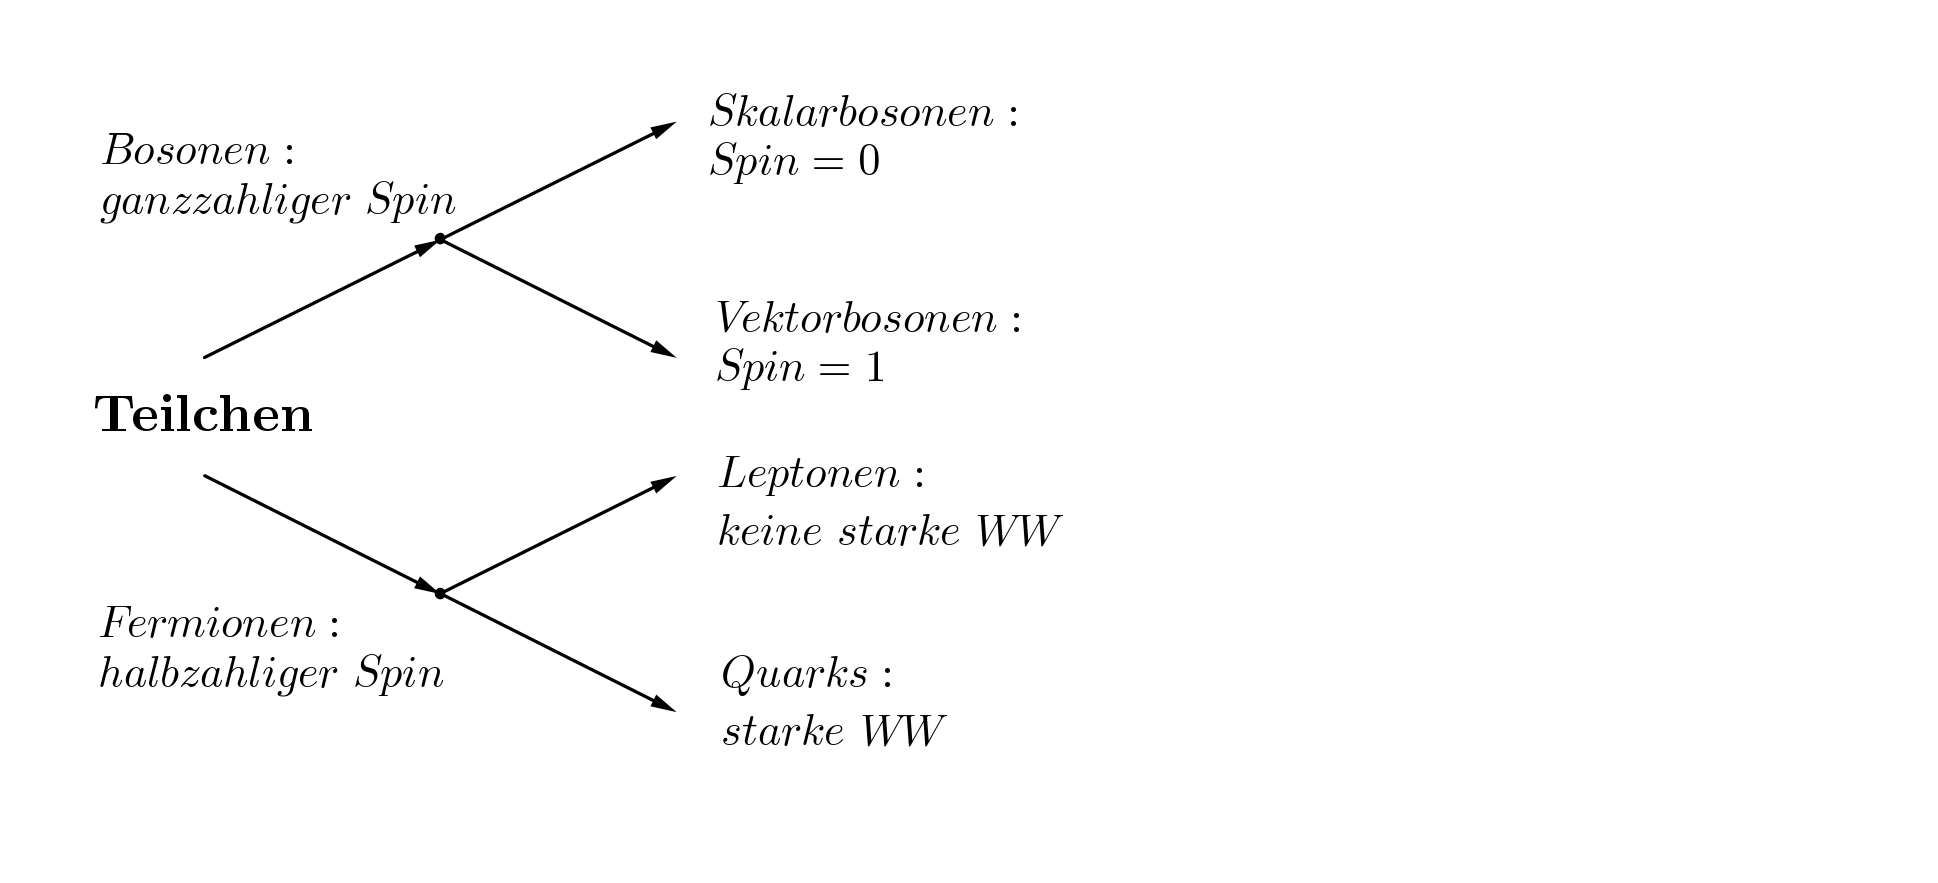
\includegraphics[width = 2\textwidth]{../Abbildungen/Teilchen.png}
%   \end{figure}
%   \end{minipage}
 \end{frame}
% 
% \begin{frame}
%  \frametitle{Feynmangraph}
%   \setcounter{framenumber}{4}
% \begin{minipage}[h]{0.38\textwidth}
%  \begin{enumerate}
%   \item ruhendes $D$-Meson
%  \end{enumerate}
% \end{minipage}
% \begin{minipage}[h]{0.58\textwidth}
%   \begin{figure}[h]
%   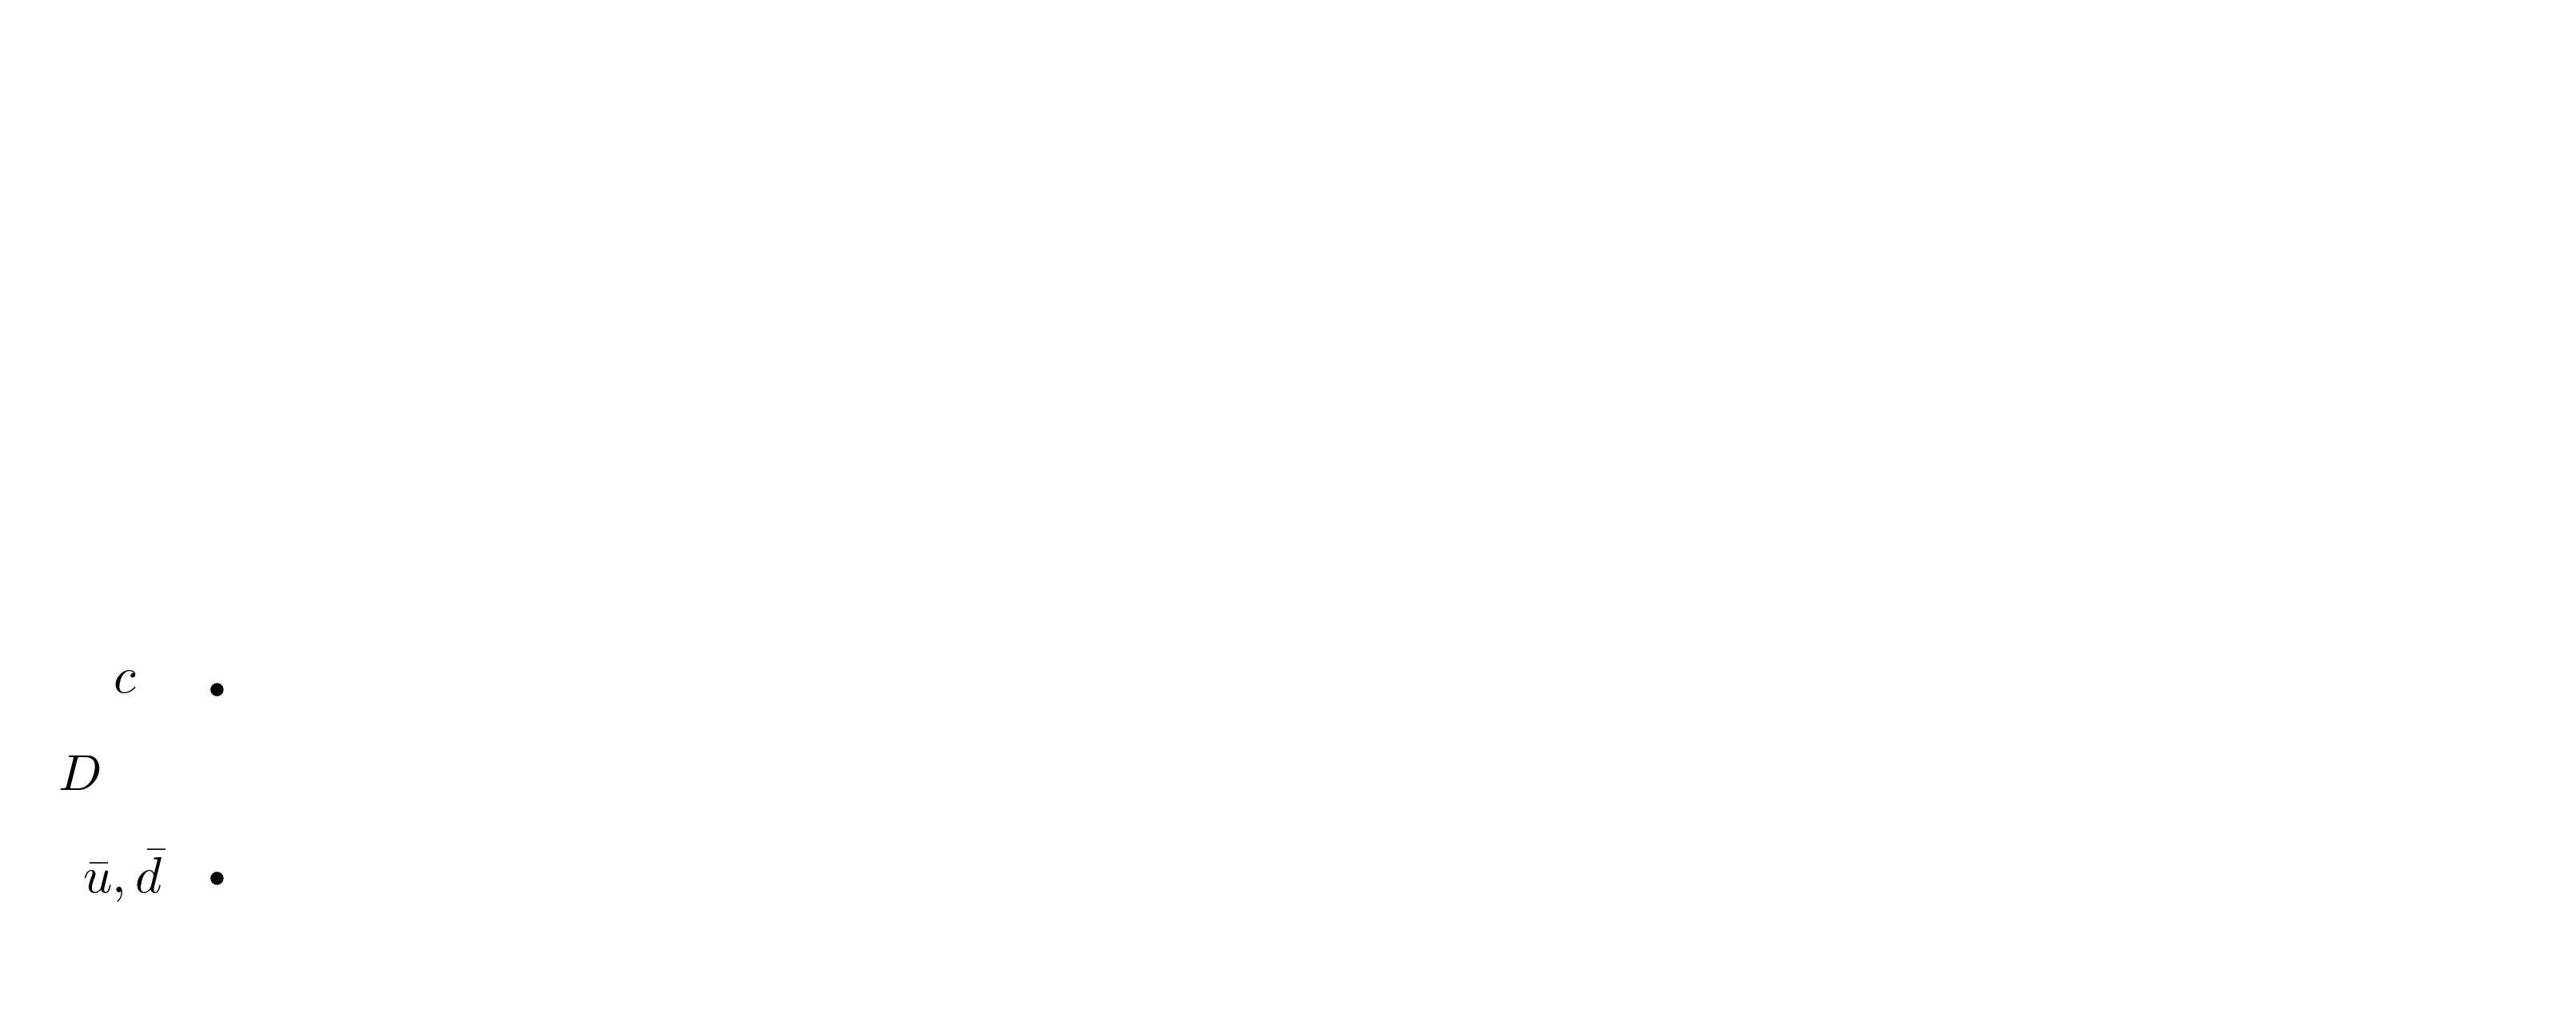
\includegraphics[width = 1.9\textwidth]{../Abbildungen/DFeyn1.png}
%    \caption{Feynmangraph des $D\rightarrow Kl\nu$ Zerfalls}
%  \end{figure}
% \end{minipage}
% \end{frame}
% 
% \begin{frame}
%  \frametitle{Feynmangraph}
% \setcounter{framenumber}{4}
% \begin{minipage}[h]{0.38\textwidth}
%  \begin{enumerate}
%   \item ruhendes $D$-Meson
%   \item propagiert in $t$
%  \end{enumerate}
% \end{minipage}
% \begin{minipage}[h]{0.58\textwidth}
%   \begin{figure}[h]
%   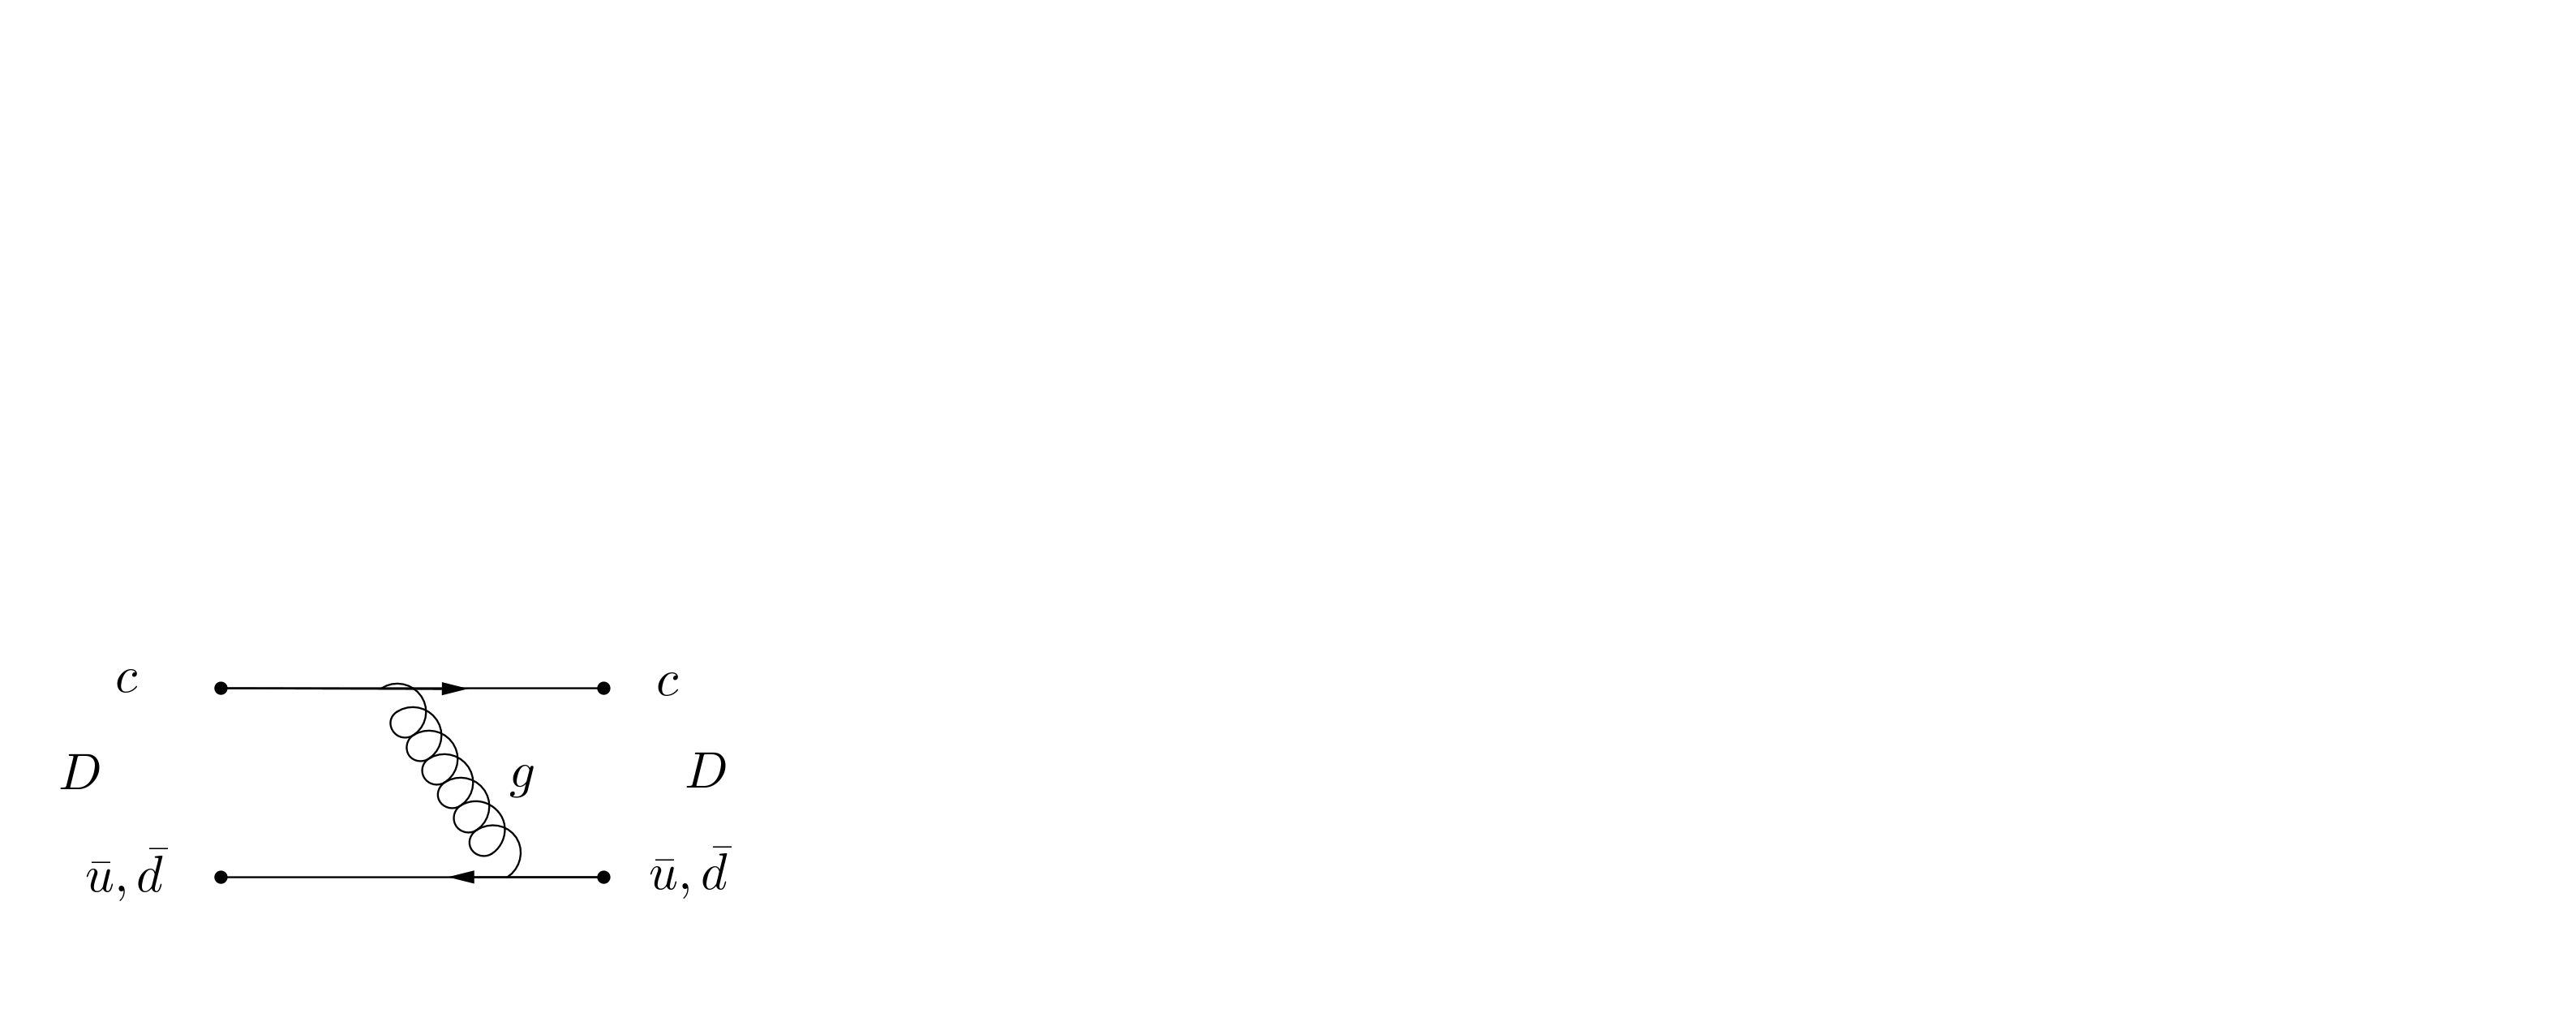
\includegraphics[width = 1.9\textwidth]{../Abbildungen/DFeyn2.png}
%    \caption{Feynmangraph des $D\rightarrow Kl\nu$ Zerfalls}
%  \end{figure}
% \end{minipage}
% \end{frame}
% 
% \begin{frame}
%  \frametitle{Feynmangraph}
%  \setcounter{framenumber}{4}
% \begin{minipage}[h]{0.38\textwidth}
%  \begin{enumerate}
%   \item ruhendes $D$-Meson
%   \item propagiert in $t$.
%   \item $c$ wandelt unter Abstrahlung von $W^+$ in $s$ 
%  \end{enumerate}
% \end{minipage}
% \begin{minipage}[h]{0.58\textwidth}
%   \begin{figure}[h]
%   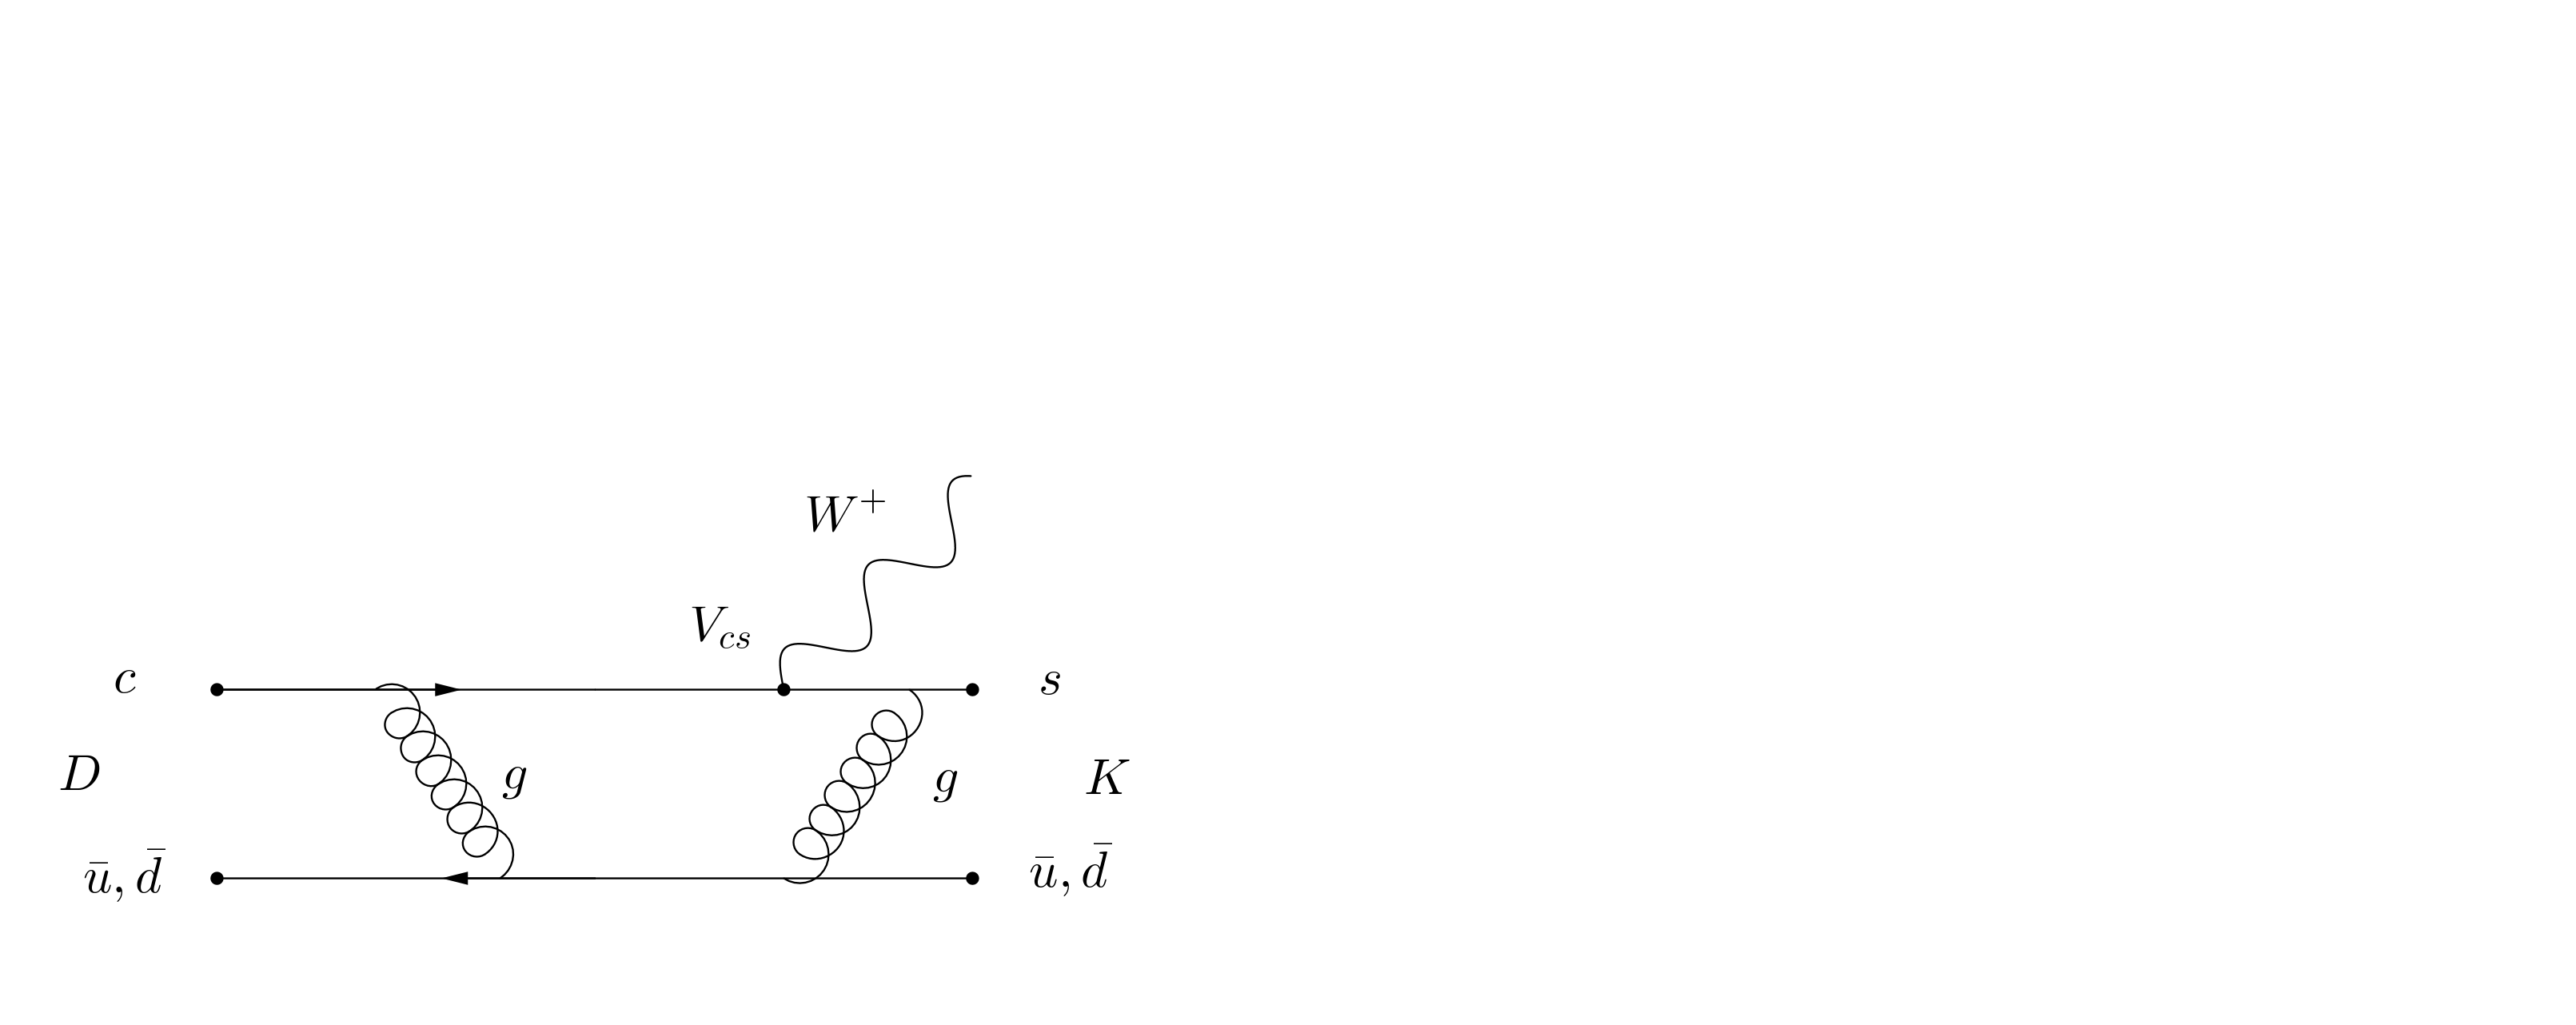
\includegraphics[width = 1.9\textwidth]{../Abbildungen/DFeyn3.png}
%    \caption{Feynmangraph des $D\rightarrow Kl\nu$ Zerfalls}
%  \end{figure}
% \end{minipage}
% \end{frame}
% 
% \begin{frame}
%  \frametitle{Feynmangraph}
%  \setcounter{framenumber}{4}
% \begin{minipage}[h]{0.38\textwidth}
%  \begin{enumerate}
%   \item ruhendes $D$-Meson
%   \item propagiert in $t$.
%   \item $c$ wandelt unter Abstrahlung von $W^+$ in $s$
%   \item $W^+$ zerstrahlt in Leptonpaar $l^+$, $\nu_l$
%  \end{enumerate}
% \end{minipage}
% \begin{minipage}[h]{0.58\textwidth}
%   \begin{figure}[h]
%   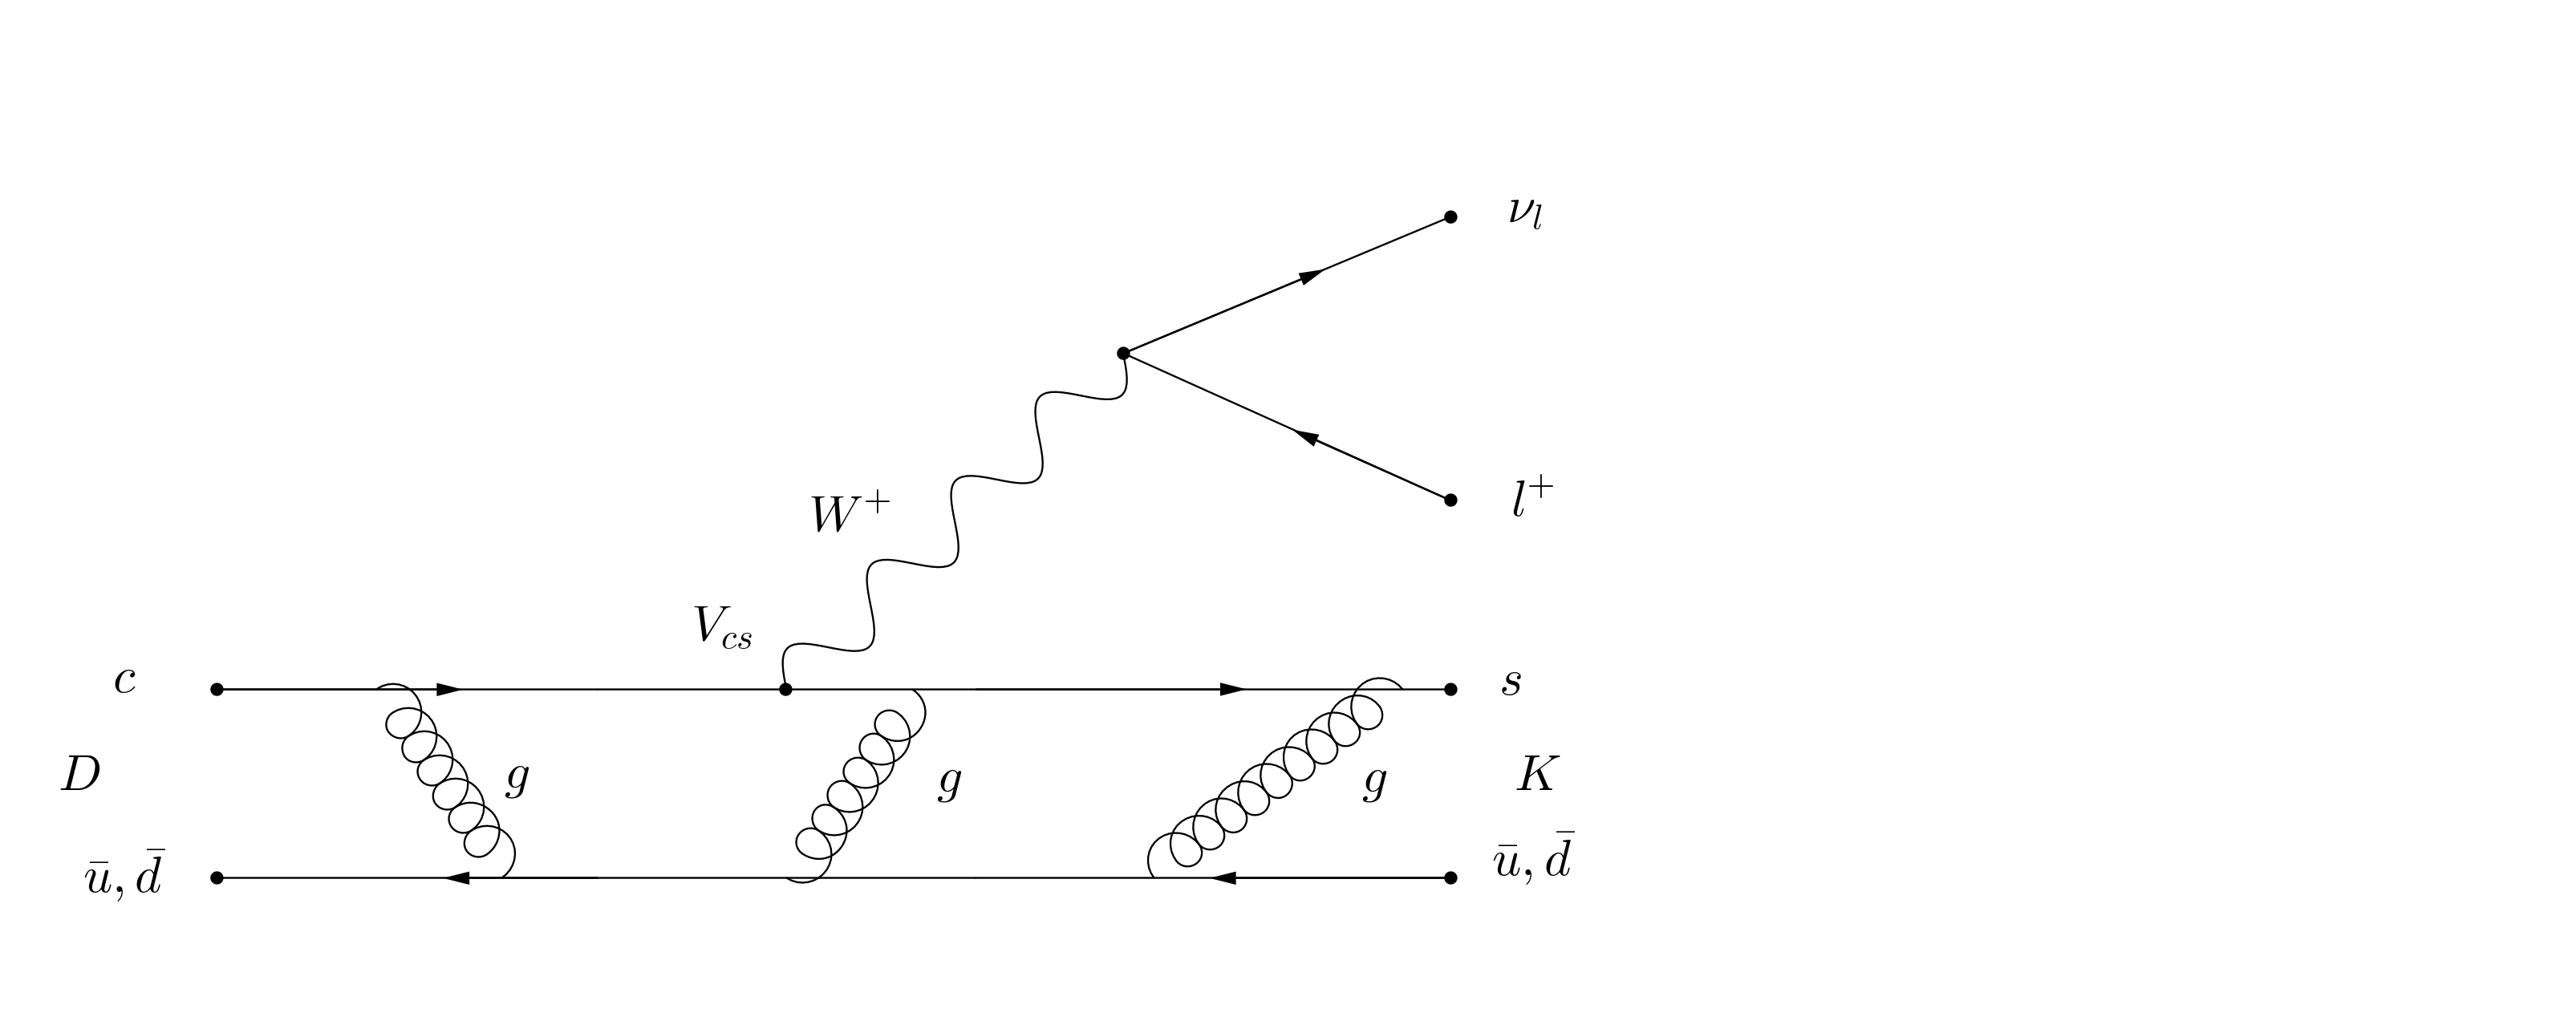
\includegraphics[width = 1.9\textwidth]{../Abbildungen/DFeyn4.png}
%    \caption{Feynmangraph des $D\rightarrow Kl\nu$ Zerfalls}
%  \end{figure}
% \end{minipage}
% \end{frame}
% 
% \begin{frame}
% \frametitle{\"Uberblick}
% \pause
%  \begin{minipage}[h]{0.62\textwidth}
%  \begin{itemize}[<+->]
%   \item Fermis Goldene Regel: $\underbrace{\Gamma}_{\text{Rate}} = 2\pi \underbrace{\delta(E_f-E_i)}_{\text{Phasenraum }\Phi}\, \cdot \,{\underbrace{|\langle f|V|i\rangle|}_{\text{Amplitude }M}}^2$
%   \item Teilchenstr\"ome
%   \begin{itemize}[<+->]
%    \item [$\circ$] relativistischer Dirac-Strom
%    \item [$\circ$] kurze Reichweite von $W^+$ f\"ur geringe Energien \\$\rightarrow$ Beschreibung durch 4-Fermionen-Wechselwirkung
%   \end{itemize}
% 
%   \item Starke WW zwischen $c$ und $\bar q_1$
%   \begin{itemize}[<+->]
%    \item[$\circ$] erh\"alt Parit\"at $\mathcal{P}$
%    \item[$\circ$] st\"orungsrechnerisch nicht erfassbar \\$\rightarrow$ Darstellung durch \textbf{Formfaktoren} $f$
%   \end{itemize}
%  \end{itemize}
% \end{minipage}
% \visible<1->{\begin{minipage}[h]{0.34\textwidth}
%   \begin{figure}[h]
%   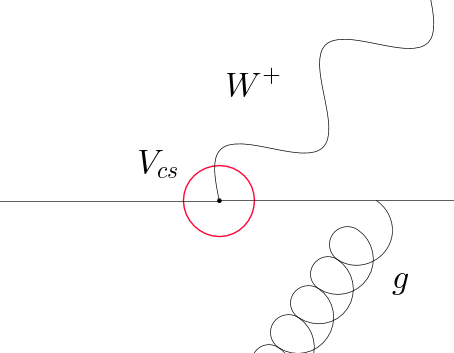
\includegraphics[width = 1.3\textwidth]{../Abbildungen/DFeynSpez.png}
% %    \caption{Feynmangraph des $D\rightarrow Kl\nu$ Zerfalls}
%  \end{figure}
% \end{minipage}}
% \end{frame}


\section{Fermis Goldene Regel}
\begin{frame}
\tableofcontents[currentsection]
\end{frame}
\subsection{Differentielle Zerfallsbreite d$\Gamma$}
 \begin{frame}
    \frametitle{Zerfallsbreite}
%    \pause
%    \begin{itemize}
%     \visible<2->{\item Inverses der hier sehr kurzen Lebensdauer $\tau$}
%     \visible<3->{\item Energiemessung führt wegen Energieunschärfe zu Verteilungen}
%     \visible<4->{\item [$\rightarrow$] Breite der Verteilung $\Gamma$ kann gemessen werden}
%     \end{itemize}
 \end{frame}

\begin{frame}
 \frametitle{Ergebnis der differentiellen Zerfallsbreite}
% Fermis Goldene Regel:\\
% \pause
% \begin{align*}
% \visible<2->{\mathrm{d} \Gamma(D\rightarrow Kl\nu) &= \frac{|M|^2}{2m_D} \mathrm{d}\Phi(K,\,l,\,\nu)} \nonumber\\
% \visible<3->{&= \frac{G_F^2 |V_{cs}|^2}{24\pi^3}|f_+(q^2)|^2|p_K|^3\mathrm{d}q^2}
% \label{eq_theoGamma}
% \end{align*}
% \vskip-1.5em
% \vspace{0.5cm}
% \visible<4->
% {\small{Fermikonstante $G_F$,\\ CKM-Element $V_{cs}$,\\ Formfaktor $f_+$,\\Kaonimpuls $p_K$,\\ Impuls\"ubertrag $q^2$}}
\end{frame}



\subsection{Phasenraumvolumen d$\Phi$}
\begin{frame}
\frametitle{Phasenraumvolumen}
% \begin{itemize}
%  \visible<2->{\item Enthält kinematische Informationen (Energien, Impulse)}
%  \visible<3->{\item Je mehr Endzustände existieren, umso größer ist $\Phi$}
%  \visible<4->{\item Nicht vom Matrixelement unabhängig ausdrückbar, da es Viererimpulse enthält}
% \end{itemize}
% \visible<5->{Ein erster Ausdruck:
% \begin{align*}
%  \mathrm{d} \Phi & = (2\pi)^4\frac{\mathrm{d}^3p_K}{2(2\pi)^3E_K} \frac{\mathrm{d}^3k_1}{2(2\pi)^3E_1} \frac{\mathrm{d}^3k_2}{2(2\pi)^3E_2}\delta^4(p_D-p_K-k_1-k_2)\nonumber
% \end{align*}}

\end{frame}

\subsection{Matrixelement $M$}
\begin{frame}
\frametitle{Matrixelement}
% \pause
% \begin{itemize}
%  \visible<2->{\item Enthält dynamische Informationen (Wechselwirkungen)}
%  \visible<3->{\item Beschreibt Übergang ähnlich Streuung von Startzustand $i$ zu Endzustand $f$}
%  \visible<4->{\item Betragsquadrat $|M|^2$ kann als Wahrscheinlichkeit für Reaktion betrachtet werden}
% \end{itemize}
%  \visible<5->{Ein erster Ausdruck:
%  \begin{align*}
%   M = \langle Kl\nu\,|\mathcal{H}|\,D\rangle
%  \end{align*}}
\end{frame}


\section{Teilchenstr\"ome}
\begin{frame}
\tableofcontents[currentsection]
\end{frame}

\subsection{Dirac-Gleichung}
\begin{frame}
\frametitle{Dirac-Gleichung}
\pause
\begin{itemize}
 \visible<2->{\item Lorentzinvariant}
 \visible<3->{\item Für Spin $\sfrac12$ -Teilchen}
 \visible<4->{\item Besitzt positiv definite Wahrscheinlichkeitsdichte $j^0$}
\end{itemize}
\visible<5-> {Dirac-Gleichung:
\begin{align*}
 (i\gamma_\mu\partial^\mu-m)\psi = (i\slashed{\partial}-m)\psi=(\slashed{p}-m)\psi = 0
 %\label{eq_dirac}
\end{align*}}
\vspace{0.5cm}

\visible<5->{\small{Dirac-Matrix $\gamma^\mu$,\\
Dirac-Wellenfunktion $\psi$,\\
Dirac-Spinoren $u$, $v$}}
\end{frame}

\begin{frame}
 \frametitle{Dirac-Strom $j^\mu$}
 \pause
 \begin{itemize}
  \visible<2->{\item Beschreibt Wahrscheinlichkeitsstrom eines propagierenden Teilchens}
  \visible<3->{\item Strom genügt Kontinuitätsgleichung $\partial_\mu j^\mu = 0$}
 \end{itemize}
\visible<4->{
 \begin{align*}
  j^\mu = \bar \psi \gamma^\mu \psi. 
 \end{align*}}
\end{frame}


\subsection{4-Fermionen-Wechselwirkung}
\begin{frame}
\frametitle{Rechtfertigung}
% \pause
%  \begin{minipage}[h]{0.58\textwidth}
% \begin{itemize}
%  \visible<2->{\item Am $W^+$ koppeln hier ein hadronischer  und ein leptonischer Strom}
%  \visible<3->{\item Hohe Masse des $W^+$ ($\approx$ 82 GeV) heißt kurze Lebensdauer
%  \begin{itemize}
%  \item[$\rightarrow$] Vier Fermionen(-ströme) wechselwirken in einem Punkt
%  \end{itemize}}
%  \visible<5->{\item Niederenergetischer Grenzfall ($q^2<2\GeV^2$) der GSW-Theorie}
% \end{itemize}
%  \end{minipage}
%  \begin{minipage}[h]{0.38\textwidth}
%  \visible<4->{\begin{figure}[h]
%   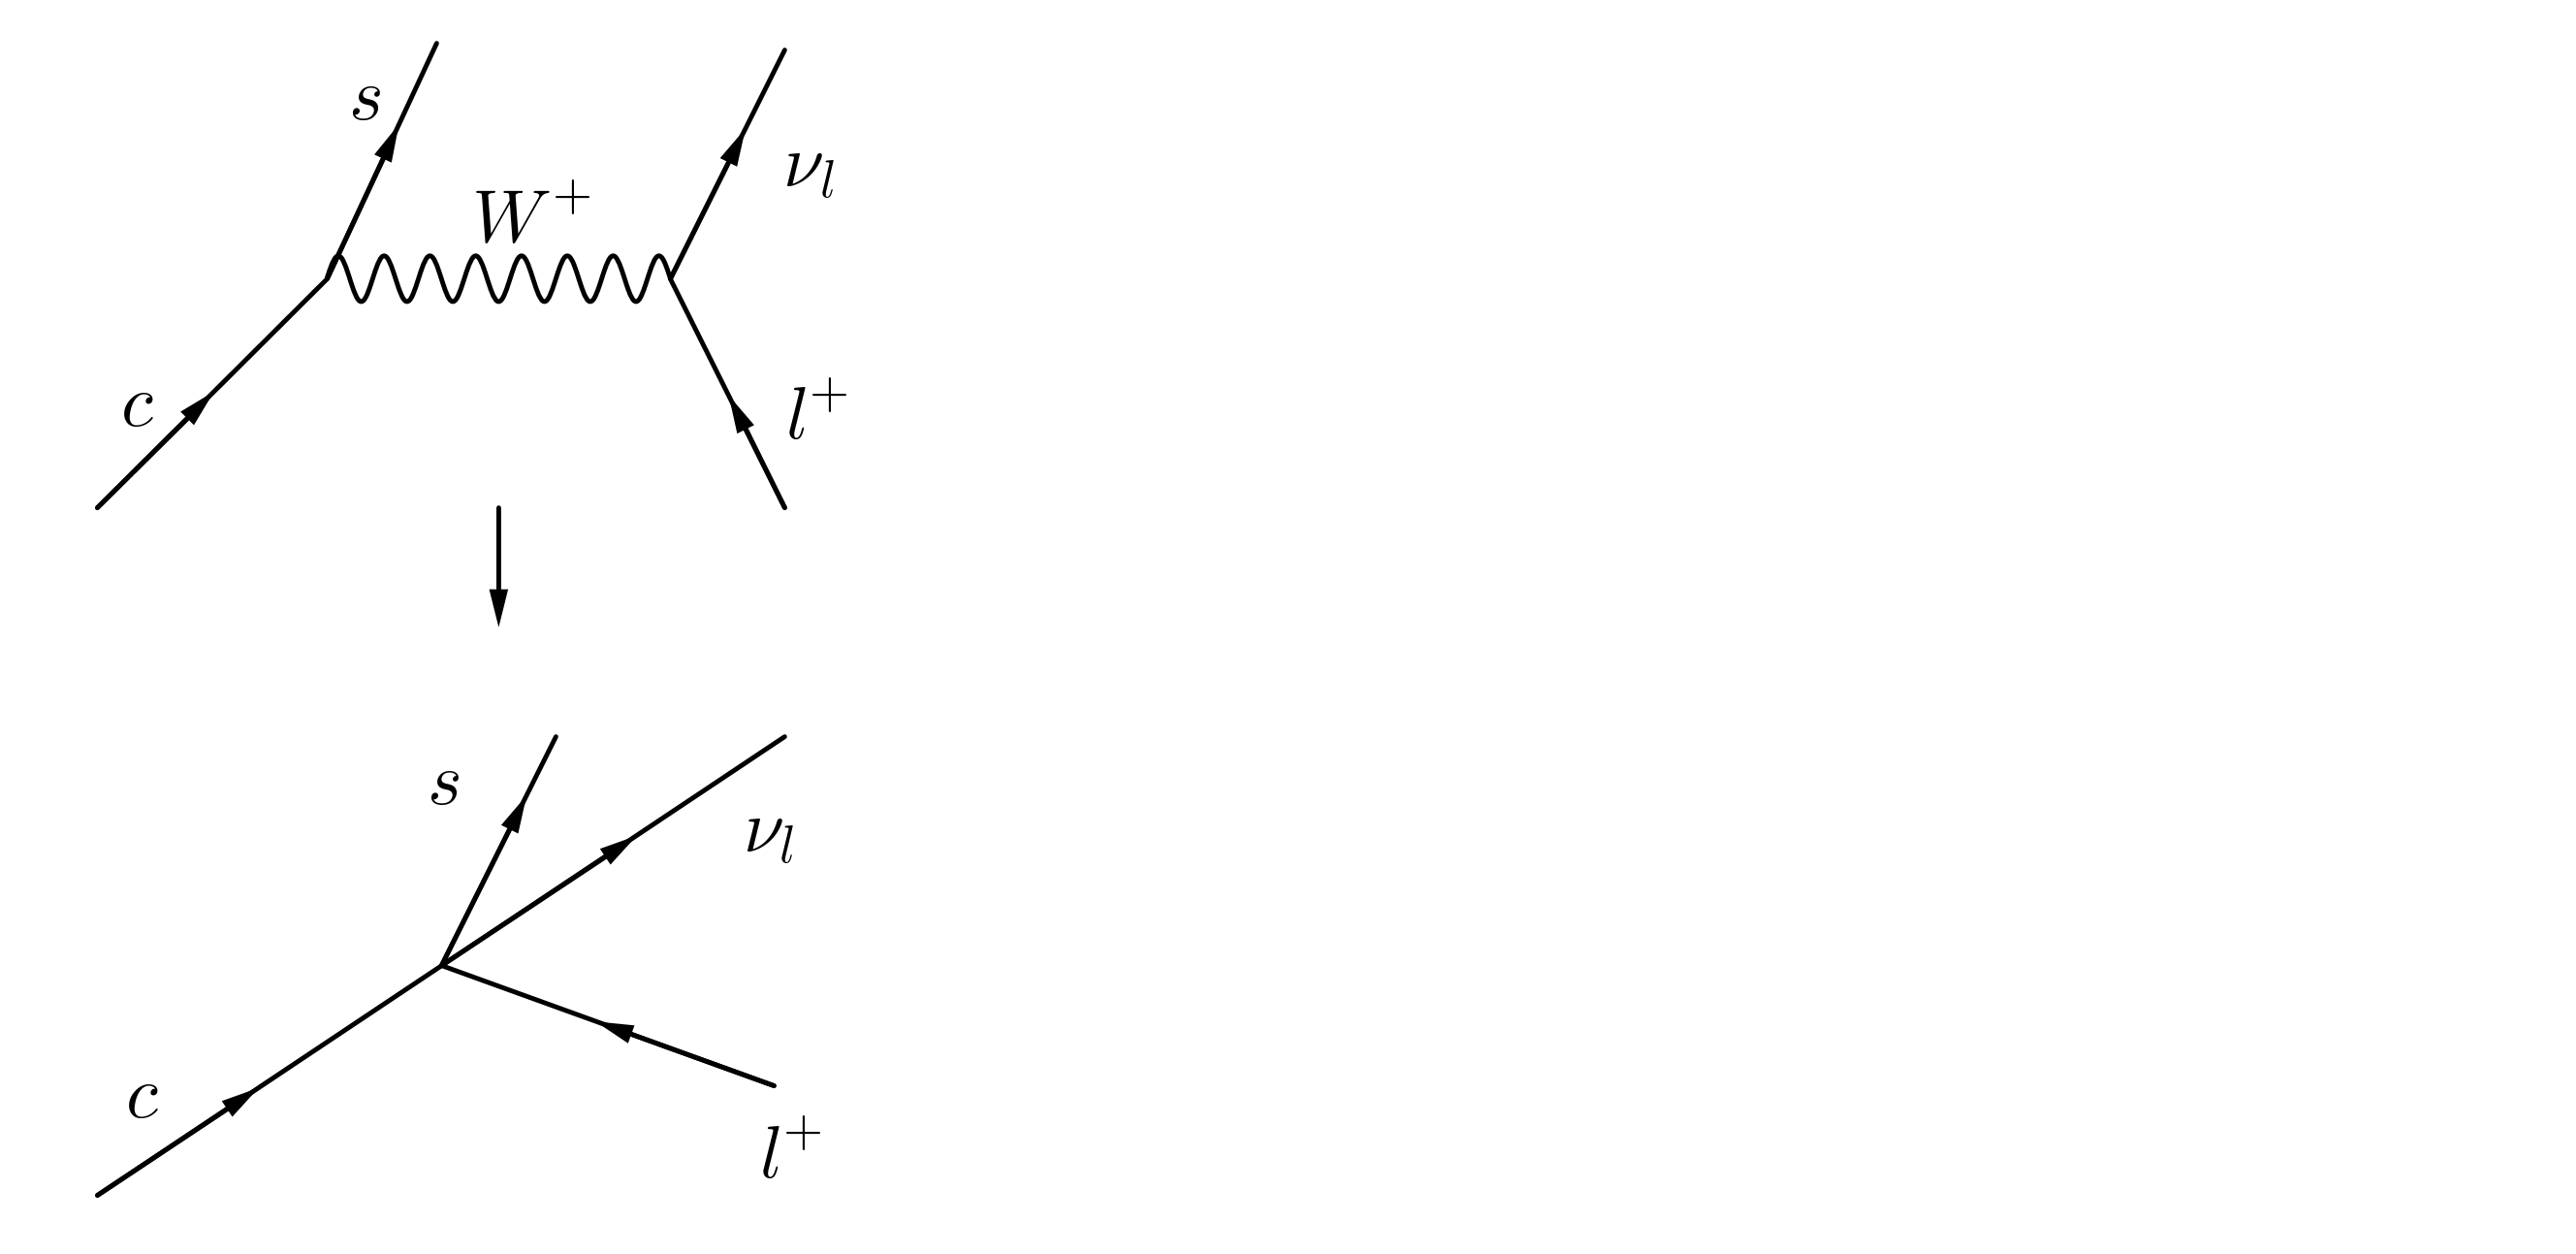
\includegraphics[width = 3\textwidth]{../Abbildungen/4FermiPraes.png}
%  \end{figure}}
%  \end{minipage}
 \end{frame}

 \begin{frame}
  \frametitle{Strom-Strom-Kopplung}
  \begin{itemize}
   \visible<2->{\item Ströme haben diverses Verhalten unter Lorentz-Transformationen (S, P, V, A, T)}
   \visible<3->{\item Experimente erfordern \textbf{Paritätsverletzung} (Schwache WW koppelt an linkshändige Teilchen und rechtshändige Antiteilchen)}
   \visible<4->{\item Dies erfordert pseudoskalaren, also kontrahierten $\mathcal{H}$ \\$\rightarrow$ Vektorstrom-Axialvektorstrom-Kopplung (V-A) }
   \visible<5->{\item Projektionsoperator $P=(1-\gamma_5)$ extrahiert linkshändige Komponente der Spinoren}
   \begin{itemize}
    \visible<6->{\item [$\rightarrow$] Dirac-Strom wird um Axialvektorstromanteil erweitert:}
   \end{itemize}
  \end{itemize}
  \visible<6->{\begin{align*}
   j^\mu = \bar \psi \gamma^\mu (1-\gamma_5) \psi
  \end{align*}}
 \end{frame}
 
% \begin{frame}
%  \frametitle{C-Matrix $V_\text{C}$}
%  \begin{itemize}
%   \item Schwache Wechselwirkung ändert Flavourquantenzahlen
%   \item Schwierigkeiten, $s$ und $c$ zu Dublett zu formen, werden durch Cabibbo-Drehung erklärt
%   \begin{itemize}
%    \item [$\rightarrow$] Darstellung des hadronischen Stroms durch Drehmatrix $V_\text{C}$
%   \end{itemize}
%  \end{itemize}
%  \begin{align*}
%   j^\mu = (\bar u \bar c)\gamma^\mu(1-\gamma_5)\underbrace{\begin{pmatrix}
% 						  \,\,\,\,\cos \theta_c\quad \sin \theta_c\\
% 						  -\sin \theta_c\quad \cos \theta_c
% 					       \end{pmatrix}}_{V_\text{C}} \begin{pmatrix}
% 							      d\\
% 							      s
% 							      \end{pmatrix}
% \end{align*}
% 
% \vspace{1cm}
% Cabibbo-Winkel $\theta_c \approx 13^\circ$
% \end{frame}

\begin{frame}
 \frametitle{CKM-Matrix $V_\text{CKM}$}
 \pause
 \begin{itemize}
  \visible<2->{\item Schwache WW ändert Flavourquantenzahlen und \textbf{verletzt CP}}
  \visible<3->{\item Ausdruck für Übergangswahrscheinlichkeit von Quarks in Form }
 \end{itemize}
 
 \begin{align*}
 V_{\text{CKM}} = \begin{pmatrix}
			    1-\frac12\lambda^2 & \lambda & \lambda^3A(\rho-\text{i}\eta)\\
			    -\lambda & 1-\frac12 \lambda^2 &\lambda^2A\\
			    \lambda^3A(1-\rho-\text{i}\eta) &-\lambda^2A & 1
			    \end{pmatrix} \, +  \, \mathcal{O}(\lambda^4)
\end{align*}
\begin{itemize}
 \item $V_{\text{CKM}}$ enthält nun komplexe Phase zur Erklärung der CP-Verletzung
 \item und drei Eulerwinkel $\theta_{12} = \theta_c,\, \theta_{13}$ und $\theta_{23}$
\end{itemize}

\vspace{0.4cm}
\small{$\lambda = \sin\theta_{12} \approx 0,2$ ,\\ $A\lambda^2 = \sin\theta_{23}$, \\ $A\lambda^3(\rho-\text{i}\eta) = \sin\theta_{13}\mathbf{e}^{-\text{i}\phi}$}
\end{frame}



\section{Formfaktoren}
\begin{frame}
\tableofcontents[currentsection]
\end{frame}
\begin{frame}
 \frametitle{Motivation}
 \begin{itemize}
  \item Fermi-Wechselwirkung berücksichtigt die starke WW zwischen $c$ und $\bar q_1$ nicht
  \begin{itemize}
   \item [$\rightarrow$] gilt aber für Leptonenstrom
   \item [$\rightarrow$] Hadronenstrom durch Formfaktoren darstellen
  \end{itemize}
  \item Formfaktoren sind einheitenlose Größen, die theoretisch unzugängliche Einflüsse enthalten (sollen berechnet werden)
  \item Viererimpulse $p_D$ und $p_K$ sind einzige Freiheitsgrade und müssen zur Darstellung ausreichen
  \item Da QCD Parität erhält, müssen Formfaktorausdrücke dasselbe Transformationsverhalten unter Parität haben, wie $V$ bzw. $A$.
 \end{itemize}
\end{frame}

\subsection{Axialvektorformfaktoren und $f_-$}
\begin{frame}
\frametitle{Axialvektorformfaktoren}
\begin{itemize}
 \item Eigenwerte der Parität $\mathcal{P}$ sind $\pi = \pm1$ und multiplikativ, da diskrete Symmetrie
 \item Vektoren und Pseudoskalare transformieren mit $\pi = -1$, Axialvektoren mit $\pi = +1$
\end{itemize}
\begin{align}
 \mathcal{P} \, \big\langle\bar K^0\,\big|V^\mu|\,D^+\big\rangle &= (-1)\cdot(-1)\cdot(-1) = -1 \nonumber \\
 \mathcal{P} \, \big\langle\bar K^0\,\big|A^\mu|\,D^+\big\rangle &= (-1)\cdot(+1)\cdot(-1) = +1. \nonumber
\end{align}
\begin{itemize}
 \item Keine Kombination aus $p_D^\mu$, $p_K^\mu$ und $\epsilon^{\mu\nu\alpha\beta}$ transformiert mit $\pi = +1$
 \begin{itemize}
  \item [$\rightarrow$] $\big\langle K(p_K)\,\big|A^\mu\big|\, D(p_D)\big\rangle = 0$
  \item [$\rightarrow$] Keine Axialvektorformfaktoren!
 \end{itemize}
\end{itemize}
\vspace{0.5cm}
\small{Levi-Civita-Tensor $\epsilon^{\mu\nu\alpha\beta}$}

\end{frame}

\begin{frame}
 \frametitle{Vektorformfaktoren}
Viererimpulse selbst transformieren unter Parität wie Vektoren
  \begin{itemize}
   \item [$\rightarrow$] Allgemeine Darstellung durch zwei Formfaktoren $f_+$, $f_-$:
  \end{itemize}

\begin{align*}
 \big\langle K(p_K)\,\big|V^\mu\big|\, D(p_D)\big\rangle = f_+(q^2)(p_D+p_K)^\mu + f_-(q^2)(p_D-p_K)^\mu.
\end{align*}
\end{frame}

\begin{frame}
 \frametitle{Formfaktor $f_-$}
 Betrachtung von $M_-$ nur mit $f_-$:
 \begin{align}
  M_- &= \frac{G_F V_{cs}}{\sqrt{2}} f_-(q^2)(p_D-p_K)^\mu\bar u_\nu \gamma_\mu(1-\gamma_5)v_l\nonumber\\
 &= \frac{G_F V_{cs}}{\sqrt{2}} f_-(q^2)(k_\nu+k_l)^\mu \bar u_\nu \gamma_\mu(1-\gamma_5)v_l\,\nonumber\\
  &=\frac{G_F V_{cs}}{\sqrt{2}} f_-(q^2)\bar u_\nu (\slashed{k}_\nu + \slashed{k}_l) (1-\gamma_5)v_l\nonumber\\
 &\stackrel{\eqref{eq_dirac}}{=}\frac{G_F V_{cs}}{\sqrt{2}} f_-(q^2)\bar u_\nu (m_\nu + m_l) (1-\gamma_5)v_l\,.\nonumber 
 \end{align}
Die Leptonmassen sind für $l=e,\,\mu$ verglichen mit $m_D$ vernachlässigbar
\begin{itemize}
 \item [$\rightarrow$] $f_-$ liefert ebenfalls keinen Beitrag!
\end{itemize}
++link zu Matrixelement II++

\end{frame}


\subsection{Formfaktor $f_+$}
\begin{frame}
 \frametitle{Kinematische Grenzen}
 Aus der Viererimpulserhaltung ergeben sich die Grenzen für $q^2$, die den Bereich für den Fit von $f_+$ angeben:
 \begin{align*}
 p_D^\mu &= p_K^\mu + p_l^\mu + p_\nu^\mu \nonumber\\
 p_D^\mu - p_K^\mu &= q^\mu = p_l^\mu + p_\nu^\mu \nonumber\\
 \left(p_D^\mu-p_K^\mu\right)^2 &= q^2 =  (p_l^\mu + p_\nu^\mu )^2\nonumber\\
 m_D^2 + m_K^2 - 2m_DE_K &= q^2 = m_l^2 + m_\nu^2 + E_lE_\nu - |\vec p_l||\vec p_\nu|\cos(\xi).
\end{align*}
Hieraus ergeben sich bei abermals vernachlässigbaren Leptonenmassen ($E = |\vec p|$) die Bereichsgrenzen zu
\begin{align*}
 0 \leq q^2 \leq (m_D-m_K)^2.
\end{align*}

\vspace{0.7cm}
Leptonenzwischenwinkel $\xi$

\end{frame}

\begin{frame}
\frametitle{Parametrisierung}
\begin{itemize}
 \item $\mathrm{d}\Gamma \propto |f_+(q^2)|^2\mathrm{d}q^2$
 \item Bei bestimmten Energien divergiert $\Gamma$
 \begin{itemize}
  \item [$\rightarrow$] Pol-Verhalten um $q^2 = m_{D^*}^2$ (außerhalb des phys. rel. Bereichs)
 \end{itemize}
 \item Parametrisierung durch Pol und Polynomreihe in $z$ mit $|z|\stackrel{!}{<}1$
 \begin{itemize}
  \item [$\rightarrow$] Gutes Konvergenzverhalten
 \end{itemize}
\end{itemize}
\end{frame}

\begin{frame}
 \frametitle{Parametrisierung}

 \begin{minipage}[h]{0.48\textwidth}
 Eine Parametrisierung für $f_+$ mit diesen Eigenschaften lautet:
\begin{align*}
 &f_+(q^2) = \frac{1}{1-\frac{q^2}{m_{D^*}^2}} \sum\limits_{i=0}^\infty a_i\,z^i(t_0,\, q^2)\\
 &z(t_0,\, q^2)= \frac{\sqrt{t_+-q^2}-\sqrt{t_+-t_0}}{\sqrt{t_+-q^2}+\sqrt{t_+-t_0}}
\end{align*}
Wahl für $t_0 = \\t_\text{opt} = t_+(1-\sqrt{1-t_-/t_+})$ minimiert Maximalwert von $|z|$.

\vspace{0.5cm}
\small{$t_\pm$ = ($m_D \pm m_K$)$^2$,\\wählbares $t_0$: $0\leq t_0 < t_+$}
 \end{minipage}
 \begin{minipage}[h]{0.40\textwidth}
 \begin{figure}
  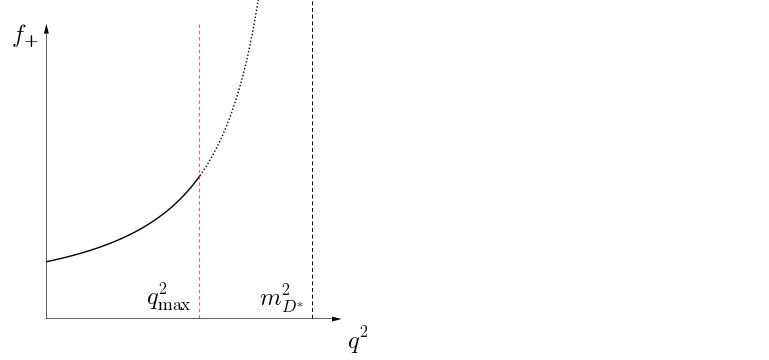
\includegraphics[width=2.7\textwidth]{../Abbildungen/formMuster.png}
 \end{figure}
 \end{minipage}
\end{frame}


\begin{frame}
 \frametitle{Methode der kleinsten Quadrate}
 \begin{itemize}
  \item Fitfunktionen weisen Abweichungen von Messwerten auf
  \item Die quadrierten Abweichungen werden aufsummiert als $\chi^2$ bezeichnet
  \begin{itemize}
   \item [$\rightarrow$] Fitparameter werden variiert, bis $\chi^2$ minimal ist
  \end{itemize}
 \end{itemize}
 Die hier verwandte $\chi^2$-Funktion lautet
 \begin{align*}
  \chi^2 = \sum\limits_{i,j=1}^m (\Delta \Gamma_i - g_i(f_+))C^{-1}_{ij}(\Delta \Gamma_j - g_j(f_+))
 \end{align*} 
 und wird durch ein \texttt{Python}-Skript unter Verwendung des Minimierungsmoduls \texttt{Minuit} vom CERN minimiert.
\end{frame}

\begin{frame}
 \frametitle{Methode der kleinsten Quadrate}
  \begin{align*}
  \chi^2 = \sum\limits_{i,j=1}^m (\Delta \Gamma_i - g_i(f_+))C^{-1}_{ij}(\Delta \Gamma_j - g_j(f_+))
 \end{align*}
 \begin{itemize}
  \item Anzahl diskreter Intervalle $m$
  \item experimentell erfasste Daten $\Delta \Gamma$
  \item theoretische Werte $g = \frac{G_F^2 |V_{cs}|^2}{24\pi^3}\int|p_K(q_i^2)|^3 \cdot |f_+(q^2_i)|^2 \mathrm{d} q_i^2$
  \item Kovarianzmatrix $C = C^{\text{stat}} + C^{\text{sys}}$; $C^{\alpha}_{ij} = \sigma^{\alpha}_i \sigma^{\alpha}_j \cdot \rho^{\alpha}_{ij}$\\ 
  $\alpha = \text{stat, sys}$; Varianzen $\sigma$; Korrelationsmatrix $\rho$  
 \end{itemize}
\end{frame}





\section{Resultate für $f_+$}
\begin{frame}
\tableofcontents[currentsection]
\end{frame}

\begin{frame}
 \frametitle{Vorbereitung}
 einleitung
\end{frame}

\begin{frame}
 \frametitle{Variation in $t_0$}
 fitresultate direkt mit angeben?
\end{frame}

\begin{frame}
 \frametitle{Variation in $\mathcal{O}$}
 fitresultate direkt mit angeben?
\end{frame}

\section{Ausblick}
\begin{frame}
\tableofcontents[currentsection]
\end{frame}

\begin{frame}
 \frametitle{Ausblick}
\end{frame}



\begin{frame}
\frametitle{Bonus}
\textbf{Bonusfolien}
\end{frame}

% \begin{frame}
%  \frametitle{Berechnung der differentiellen Zerfallsbreite}
%  
%  \begin{align}
%  \mathrm{d} \Phi & = (2\pi)^4\frac{\mathrm{d}^3p_K}{2(2\pi)^3E_K} \frac{\mathrm{d}^3k_1}{2(2\pi)^3E_1} \frac{\mathrm{d}^3k_2}{2(2\pi)^3E_2}\delta^4(p_D-p_K-k_1-k_2)\nonumber\\
%  &=\frac{1}{(2\pi)^5}\frac{\mathrm{d}^3p_K}{2E_K}\int \frac{\mathrm{d}^3k_1}{2(2\pi)^3E_1} \frac{\mathrm{d}^3k_2}{2(2\pi)^3E_2}\delta^4(q-k_1-k_2)k_{1,\mu} k_{2,\nu}\nonumber
%  \end{align}
% Leptonimpulse $k_i$ integriert, da Verteilung der Zerfallsbreiten durch $\mathrm{d}q^2$ gemessen. Die Eintr\"age $k_{1,\mu}$ und $k_{2,\nu}$ stammen von $M$ (folgt im Anschluss)
% \end{frame}
% 
% \begin{frame}
%  \frametitle{Berechnung}
%  F\"ur die weitere Berechnung werden folgende Gleichungen des $D$-Meson-Ruhesystems ben\"otigt:
%  \begin{itemize}
%  \item $ \frac{\mathrm{d}^3p_K}{2E_K} = 2\pi |p_K|\mathrm{d}E_K$
%    \item $|p_K| = \frac{\sqrt{\lambda(m_D^2, m_K^2, q^2)}}{2m_D}$
%    \item $\int \frac{\mathrm{d}^3k_1}{2(2\pi)^3E_1} \frac{\mathrm{d}^3k_2}{2(2\pi)^3E_2}\delta^4(q-k_1-k_2)k_{1,\mu} k_{2,\nu} = \frac{\pi}{24}(q^2g_{\mu\nu} + 2q_\mu q_\nu)$
%  \end{itemize}
%  \vspace{0.7cm}
%  \small{$\lambda = a^2+b^2+c^2-2(ab+bc+ac)$ - K\"all\'en-Funktion,\\$g_{\mu,\nu} = \text{diag}(1,-1,-1,-1)$ - Minkowski-Metrik}
% \end{frame}
% 
% \begin{frame}
%  \frametitle{Berechnung}
%  Diese f\"uhren zu einem Ausdruck f\"ur das Phasenraumvolumen:
%  \begin{align}
%   \mathrm{d}\Phi = \frac{\pi}{24}(q^2g_{\mu\nu} + 2q_\mu q_\nu)\frac{|p_K|}{(2\pi)^4}\mathrm{d}E_K
%  \end{align}
% \end{frame}
% 
% \begin{frame}
%  \frametitle{Berechnung II}
%  Abschliessend kann das quadrierte Matrixelement nach Umformung des leptonischen Anteils durch Casimirs Trick wie folgt geschrieben werden als
%  \begin{align}
%   |M|^2 & = \frac{G_F^2|V_{cs}|^2}{2}|f_+(q^2)|^2 P^\mu P^\nu \cdot 8\big(k_{l,\mu} k_{\nu,\nu} - g_{\mu\nu}k_lk_\nu + k_{l,\nu}k_{\nu,\mu}\big)\nonumber\\
%   & = 4G_F^2|V|^2 |f_+(q^2)|^2 \big(2P^\mu P^\nu - P^2 g^{\mu\nu}\big) k_{l,\nu}k_{\nu,\mu}
%   \label{eq_theoAmplitude}
%  \end{align}
% \end{frame}
% 
% \begin{frame}
% \frametitle{Berechnung II}
%  Nun k\"onnen \eqref{eq_theoPhase} und \eqref{eq_theoAmplitude} unter Verwendung von
%  \begin{align*}
%  \big(2P^\mu P^\nu - P^2 g^{\mu\nu}\big)\big(2q_\mu q_\nu + q^2g_{\mu\nu}) = 4 \lambda(m_D^2,m_K^2,q^2) = 16 m_D^2 |p_K|^2
%  \end{align*}
%  miteinander verkn\"upft und zu \eqref{eq_theoGamma} zusammengefasst werden
%  ++Verlinkung auf f++
% 
% \end{frame}




\end{document}
